% Licensed under the Creative Commons Attribution Share Alike 4.0 International.
% See the LICENSE file in the repository root for full license text.

\section{通过 GUI 使用 CMake}

\begin{figure}[p]
	\centering
	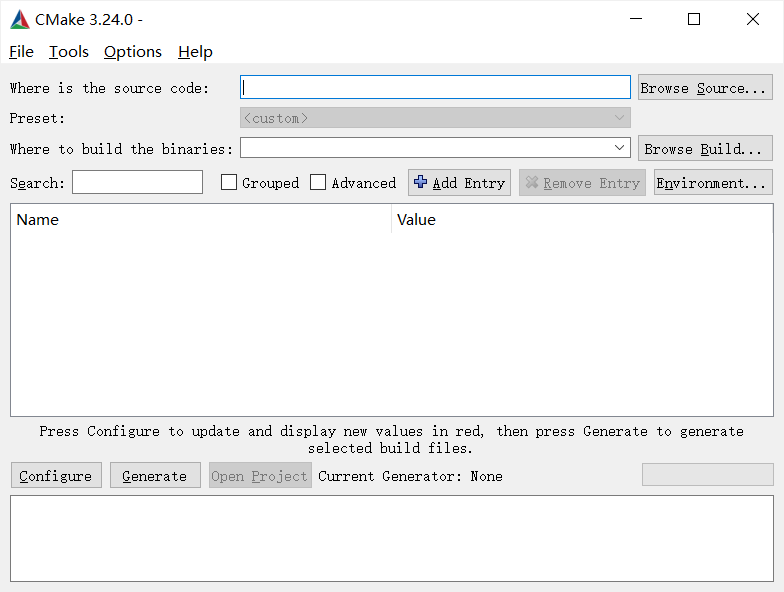
\includegraphics[width=0.75\linewidth]{assets/cmake-gui-1}
	\caption{cmake-gui 程序的窗口。}
	\label{fig:cmake-gui-1}
\end{figure}

\begin{figure}[p]
	\centering
	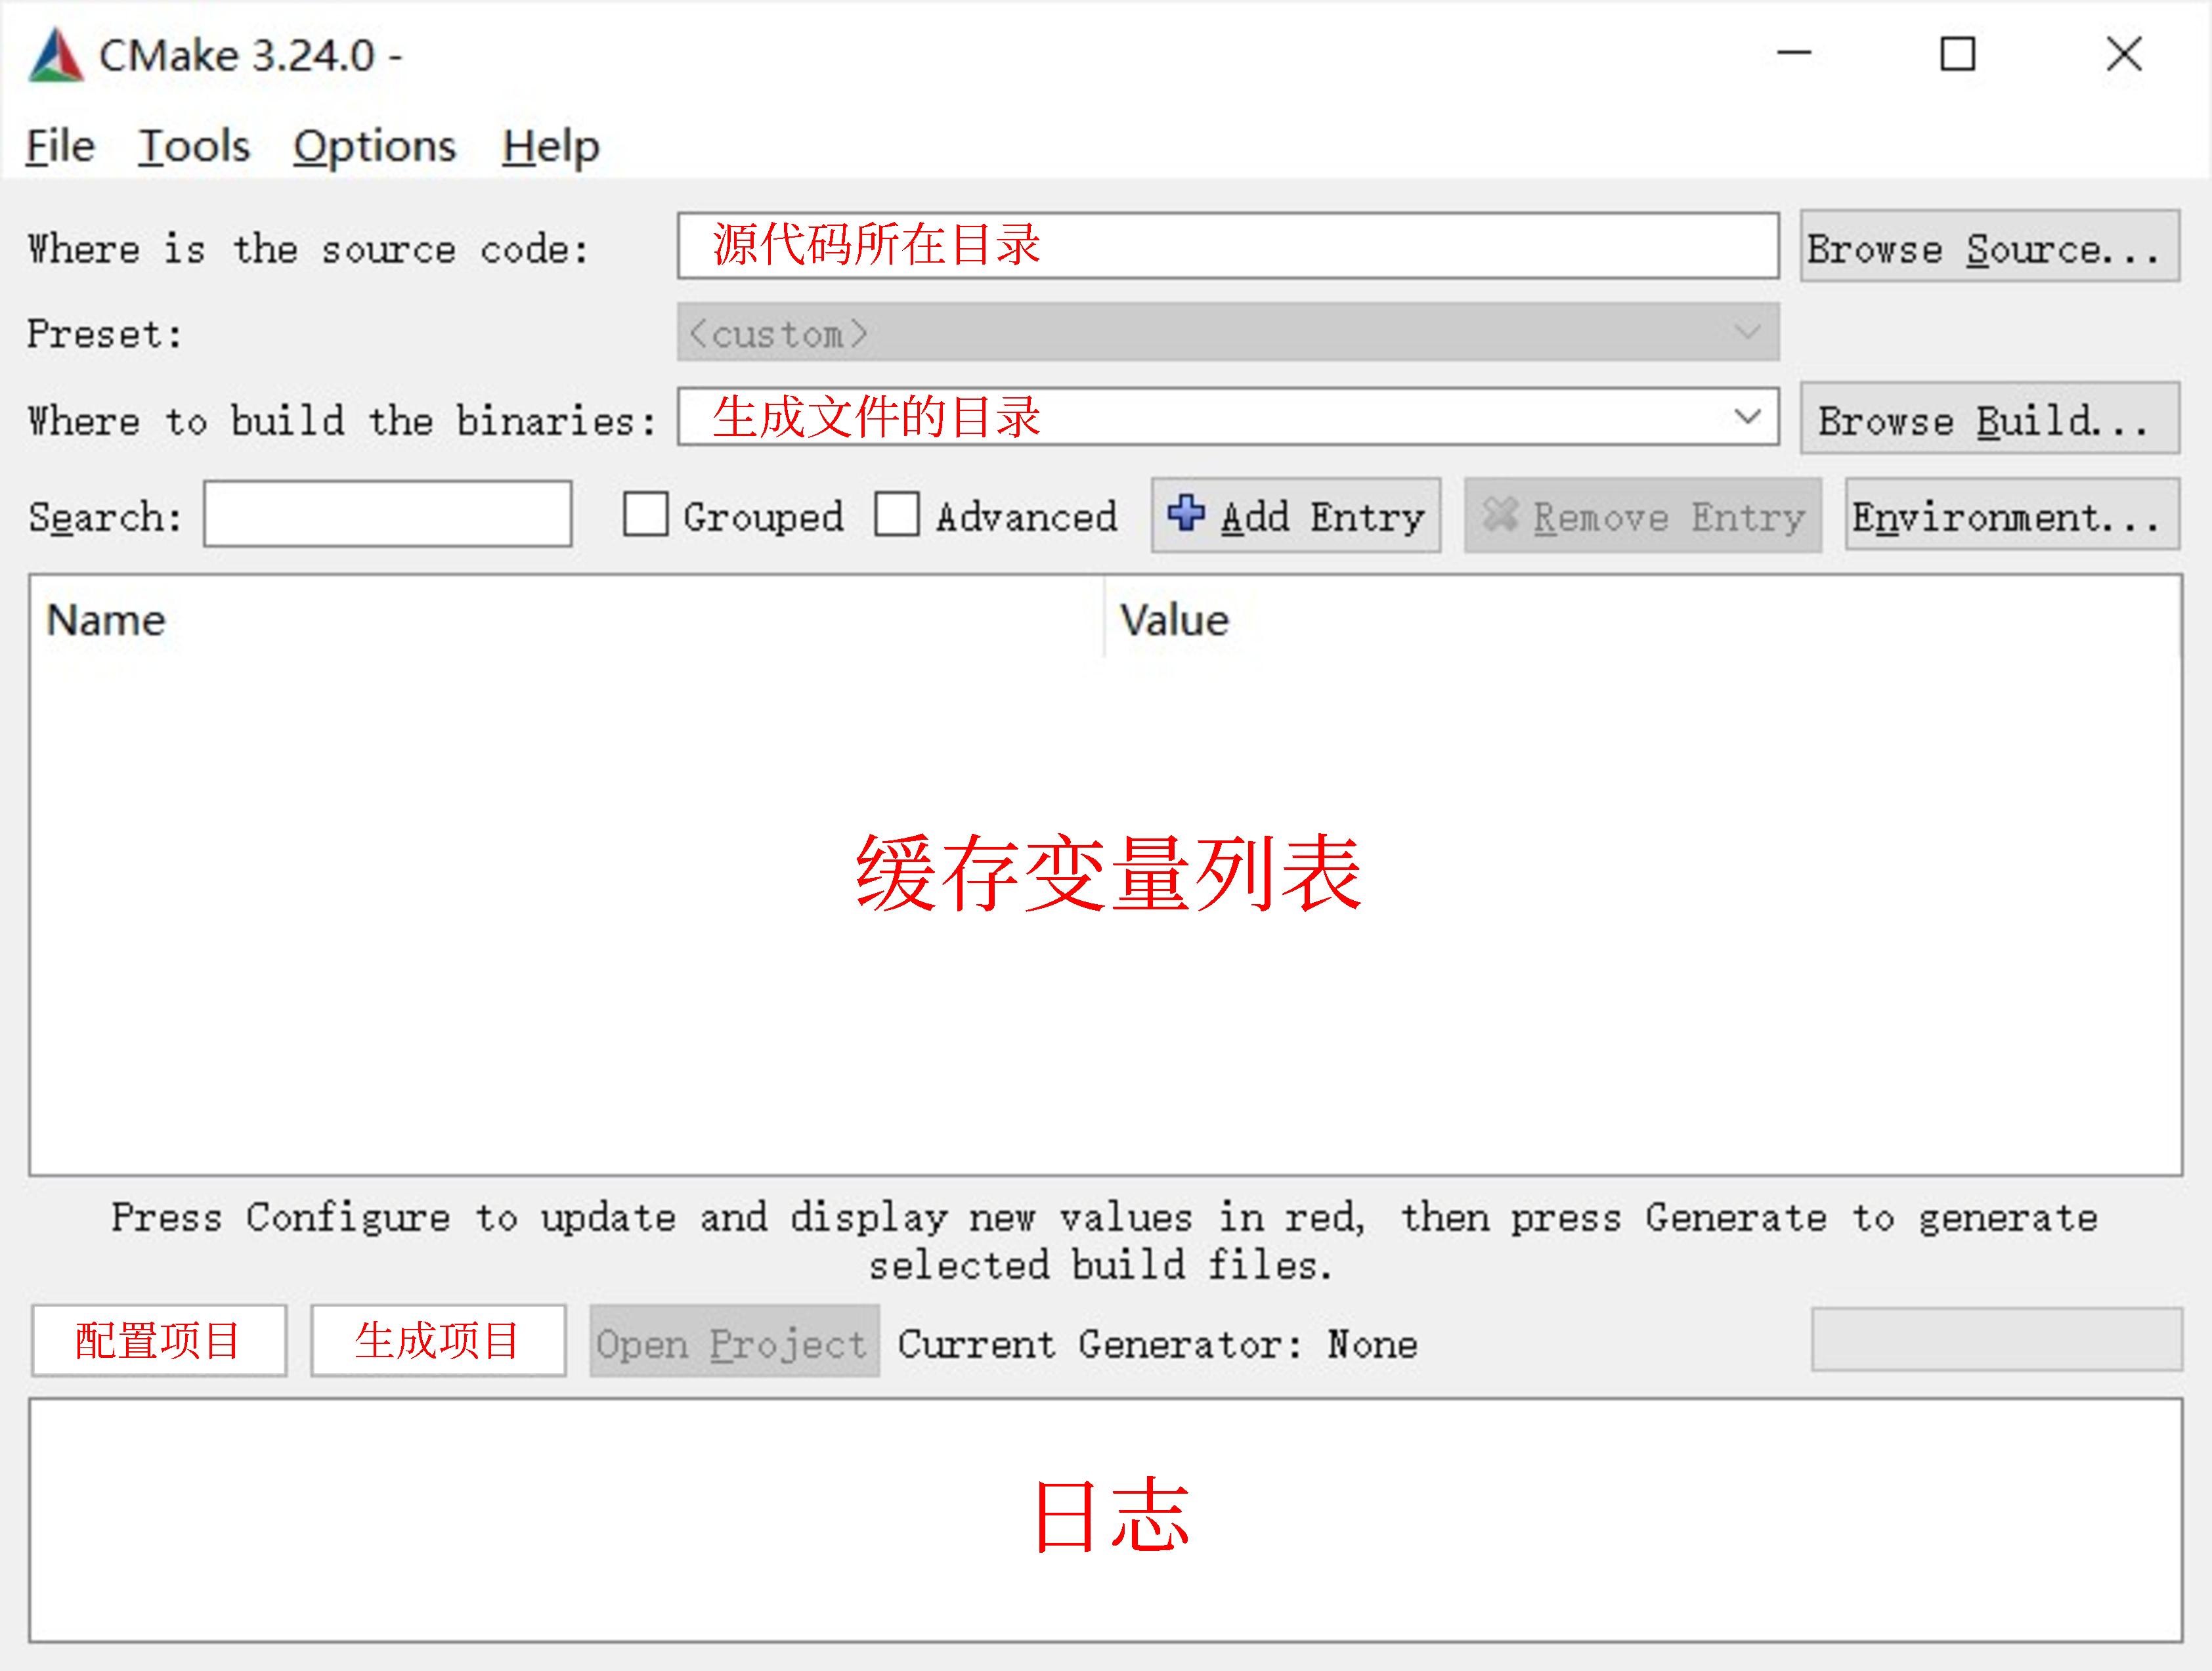
\includegraphics[width=0.75\linewidth]{assets/cmake-gui-2}
	\caption{cmake-gui 窗口解释。}
	\label{fig:cmake-gui-2}
\end{figure}

安装的 CMake 附带了一个\emph{图形用户界面(graphics user interface,GUI)}应用程序,名为 cmake-gui。从开始菜单依次打开“CMake”“CMake (cmake-gui)”,将显示图 \ref{fig:cmake-gui-1} 所示的窗口。

图 \ref{fig:cmake-gui-2} 解释了该窗口中各部分的含义。图中最抢眼的是中间的列表控件,它被称为\emph{缓存变量(cached variable)}列表。缓存变量将允许我们自定义项目的一些选项。CMake 将缓存变量的值保存在生成的一个临时文件 \lstinline[language={}]{CMakeCache.txt} 中,我们可以借助 cmake-gui 的这个列表控件方便地修改它们。一般而言,一旦缓存变量文件被生成,缓存变量的值就不会随 CMake 的运行而改变,它们将一直采用缓存变量文件保存的值:所以在之后的实验过程中,如果总是出现未知的错误,不妨删除 \lstinline[language={}]{CMakeCache.txt} 后再试一次。

% TODO: 把“下一章”替换为“第 n 章”,其他同理。

我们将在下一章中详细讲解缓存变量的相关知识。除了配置缓存变量这一功能,cmake-gui 还能帮助我们调用真正的 CMake 程序,对应图 \ref{fig:cmake-gui-2} 中的“配置项目”“生成项目”按钮,我们将在下一节讲解它们的作用。由于 cmake-gui 的本质是帮助我们修改文本文件、调用命令行,而市面上大量的 IDE 都已很好地集成了 CMake,所以在开发和自动化测试时我们一般都不使用 cmake-gui。cmake-gui 一般只用于刚刚从网络上下载的项目,这时它相比命令行可谓简而不繁。
